\chapter{Dynamic Memory Management}
\label{chp:dynamic-memory-management}
Native support of complex data structures is a non-trivial matter to implement in a reversible computing environment. Variable-sized records and frames need to be stored efficiently in a structured heap, while avoiding garbage build-up to maintain reversibility. A reversible heap manager layout has been proposed for a simplified version of the reversible functional language \textsc{RFun} and later expanded to allow references to avoid deep copying values~\cite{ha:heap, ty:rfun, tm:refcounting}.

The following section presents a discussion of various heap manager layouts along with their advantages and disadvantages in terms of implementation difficulty, garbage build-up and the OOP domain. 

\section{Fragmentation}
\label{sec:fragmentation}
An important matter to consider when designing a heap layout for dynamic memory allocation is efficient memory usage. In a stack allocating memory layout, the stack discipline is in effect, meaning only the most recently allocated data can be freed. This is not the case with heap allocation, where data can be freed regardless of allocation order. This feature comes with the consequence of potential memory fragmentation, as blocks are being freed in any order~\cite{tm:languages}.

We distinguish different types of fragmentation as internal or external fragmentation.

\subsection{Internal Fragmentation}
% TODO: Revise
Internal fragmentation occurs in the memory heap when part of an allocated memory block is unused. This type of fragmentation can arise from a number of different scenarios, but mostly it originates from \textit{over-allocating}. 

An example of \textit{over-allocating} would be a scenario where we are allocating memory for an object of size $m$ onto a simple, fixed-sized block heap, where the fixed block size is $n$ and $m \neq n$. If $n > m$, internal fragmentation would occur of size $n-m$ for every object of size $m$ allocated in said heap. If $n < m$, numerous blocks would be required for allocation to fit our object. In this case the internal fragmentation would be of size $m + n - (m + n) \mod n$ per allocated object of size $m$. 

\begin{figure}[ht]
\centering
\texttt{TODO}
\caption{Example of internal fragmentation due to \textit{over-allocation}}
\label{fig:internal-frag-example}
\end{figure}

Figure~\ref{fig:internal-frag-example} visualizes the examples of internal fragmentation build-up from \textit{over-allocating} memory. 

Intuitively, internal fragmentation can be prevented by ensuring that the size of the block(s) being used for allocating space for an object of size $m$ either match or sums to this exact size.

\subsection{External Fragmentation}
% TODO: Revise
External fragmentation materializes in the memory heap when a freed block becomes partly or completely unusable for future allocation if it, say, is surrounded by allocated blocks but the size of the freed block is too small to contain any object on its own.

This type of fragmentation is generally a more substantial cause of problems than internal fragmentation, as the size of external fragmentation blocks usually are larger than the ones created from internal fragmentation, depending on the heap implementation (In a layout using variable-sized blocks of, say, size $2^n$, the internal fragment size becomes considerable for large $n$s). 

Non-allocatable external fragments become a problem when there it is impossible to allocate space for a large object as a result of too many non-consecutive blocks scattered around the heap, caused by the external fragmentation. Physically, there is enough space to store the object, but not in the current heap state. In this scenario we would need a garbage collector to clean the heap and relocate blocks in such a manner that the fragmentation disperses.

\begin{figure}[ht]
\centering
\texttt{TODO}
\caption{Example of external fragmentation}
\label{fig:external-frag-example}
\end{figure}


\section{Memory Garbage}
\label{sec:memory-garbage}
In the reversible setting it should be our goal to return the memory to its original state after program termination.

Traditionally, in non-reversible programming languages, freed memory blocks are simply re-added to the free-list during deallocation and no modification of the actual data stored in the block is done. In the reversible setting we must return the memory block to its original state after the block has been freed (e.g. zero-cleared), to uphold the time-invertible and two-directional computational model. 

In heap allocation, we maintain one or more free-lists to keep track of free blocks during program execution, which are stored in memory, besides the heap representation itself. These free-lists can essentially be considered garbage and as such, they must also be returned to their original state after execution. Furthermore, the if the heap grows during execution, it should be returned to its original size.

Returning the free-list(s) to their original states is a non-trivial matter, which is highly dependent on the heap layout and free-list design.~\citeauthor{ha:heap} introduced a dynamic memory manager which allowed heap allocation and deallocation, but without restoring the free-list to its original state in~\cite{ha:heap}.~\citeauthor{ha:heap} argue that an unrestored free-list is to be considered harmless garbage in the sense that the free-list left after termination is equivalent to a restored free-list, as it contains the same blocks, but linked in a different order, depending on the order of allocation and deallocation operations performed during program execution.

This intuitively leads to the question of garbage classification. In the reversible setting all functions are injective. Thus, given some $input_f$, the injective function $f$ produces some $output_f$ and some $garbage_f$ (e.g. garbage in form of storing data in the heap, so the free list changes, the heap grows, etc.). Its inverse function $f^{-1}$ must thus take $f$'s $output_f$ and $garbage_f$ as $input_{f^{-1}}$ to produce its output $output_{f^{-1}}$ which is $f$'s $input_f$. However, in the context of reversible heaps, we must consider all free-lists as of "equivalent garbage class" and thus freely substitutable with each other, as injective functions still can drastically change the block layout, free-list order, etc. during its execution in either direction. Figure~\ref{fig:equivalent-free-lists} shows how any free-list can be passed between a function $f$ and its inverse $f^{-1}$.

\begin{figure}[ht]
\centering
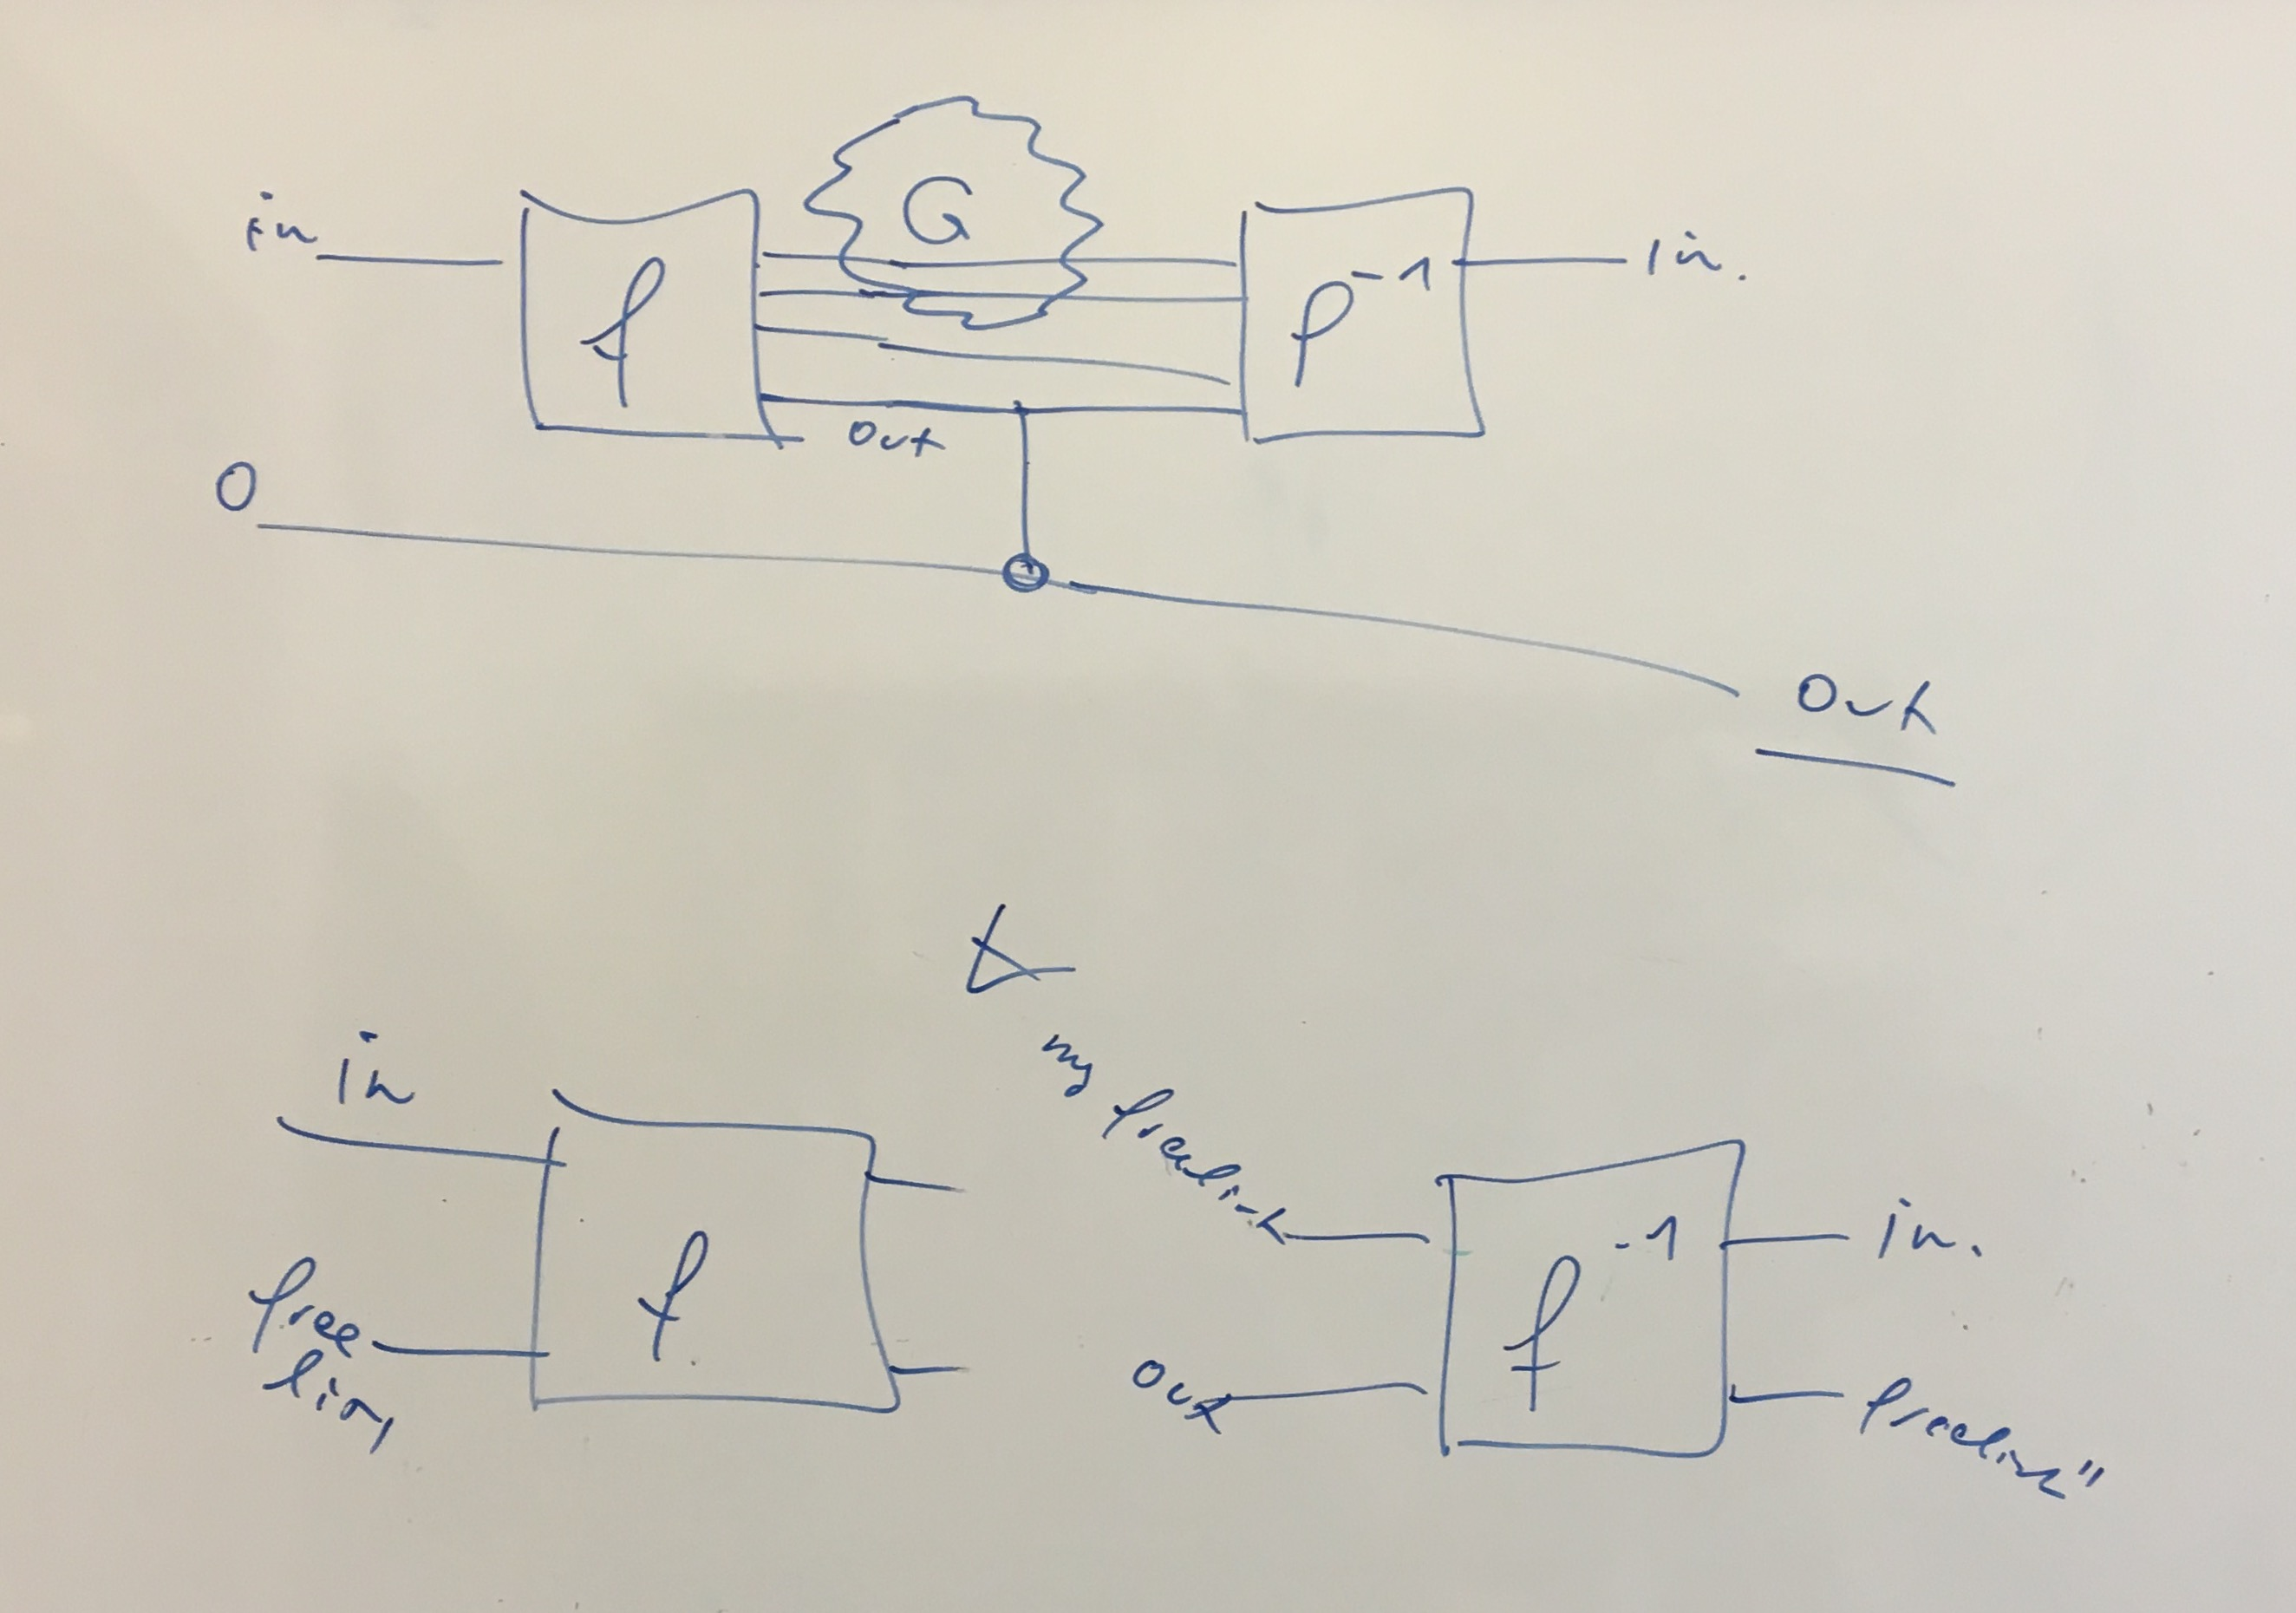
\includegraphics[width=0.7\textwidth]{garbage-classes}
\caption{All free-lists are considered equivalent in terms of injective functions (Temporary photo)}
\label{fig:equivalent-free-lists}
\end{figure}


\section{Heap manager layouts}
\label{sec:heap-manager-layout}
Heap managers can be implemented in numerous ways. Different layouts yield advantages when allocating memory, finding a free block or when collecting garbage. As our goal is to construct a garbage-free heap manager, our finalized design should emphasize and reflect this objective in particular. Furthermore, we should attempt to allocate and deallocate memory as efficiently as possible, as merging and splitting of blocks is a non-trivial problem in a reversible setting.

For the sake of simplicity, we will not consider the the issue of retrieving memory pages reversibly. A reversible operating system is a long-term dream of the reversible programmer and as reversible programming language designers, we assume that \rooplpp will be running in an environment, in which the operating system will be supplying memory pages and their mappings. As such, the following heap memory designs reflect this preliminary assumption, that we always can query the operating system for more memory. 

Historically, most object-oriented programming languages utilize a dynamic memory manager during program execution. In older, lower-level languages such as \textsc{C}, memory allocation had to be stated explicitly and with the requested size through the \texttt{malloc} statement and deallocated using the \texttt{free} statement. Modern languages, such as \textsc{C\texttt{++}}, \textsc{Java} and \textsc{Python}, \textit{automagically} allocates and frees space for objects and variable-sized arrays by utilizing their dynamic memory manager to dispatch \texttt{malloc}- and \texttt{free}-like operations to the operating system and managing the obtained memory blocks in private heap(s)~\cite{wh:cpp_memory, bv:jvm, py:memory}. The heap layout of these managers vary from language to language and compiler to compiler.

% Reversible Heaps
Previous work on reversible heap manipulation has been done for reversible functional languages in~\cite{ha:heap, jsk:translation, tm:garbage}.

% TODO: Something about Cons/Nil heap from ~\cite{ha:heap}

% TODO: Something about ref count extension~\cite{tm:refcounting}


For the sake of simplicity in the following heap layout pseudo-code outlines, we assume access to the following subroutines (with parameter passing), inspired by the body of \citeauthor{ha:heap}'s \texttt{get\_free} subroutine.

In order to reversibly allocate a block, we assume access to the subroutine \texttt{allocate\_block} which, given the register $r_{cell}$ where we want the address of the allocated block stored and the register $r_{flp}$ containing the free-list pointer, effectively pops the head of the free-list to  $r_{cell}$. Listing~\ref{lst:allocate-block-sub} shows the subroutine.

\begin{lstlisting}[caption={\texttt{allocate\_block} subroutine}, language=janus, style=basic,label={lst:allocate-block-sub}]
procedure allocate_block($r_{cell}$, $r_{flp}$)
	EXCH $r_{cell}$ $r_{flp}$
	SWAP $r_{cell}$ $r_{flp}$
\end{lstlisting}

% In order to grow the heap, we assume access to the subroutine \texttt{grow\_heap} which, given the register $r_{hp}$ containing the heap pointer and a number $n$ specifying how much the heap should grow, increments the heap pointer by $n$. Listing~\ref{lst:grow-heap-sub} shows the subroutine.

% \begin{lstlisting}[caption={\texttt{grow\_heap} subroutine}, language=janus, style=basic,label={lst:grow-heap-sub}]
% procedure grow_heap($r_{hp}$, $n$)
% 	ADDI $r_{hp}$ $n$
% \end{lstlisting}

% Finally, in order to move the heap, we assume access to the subroutine \texttt{move\_heap} which, given the register $r_{hbp}$ containing a pointer to the \textit{bottom of a heap}\footnote{assuming it exists} and the register $r_{hp}$ containing the heap pointer and a number $n$ representing the amount the heap should be moved, iterates every memory address in the heap, starting at the top, and moves the memory block $n$ spaces. This is down using a top-down approach to avoid overwriting data. 

% \begin{lstlisting}[caption={\texttt{move\_heap} subroutine}, language=janus, style=basic,label={lst:move-heap-sub}]
% procedure move_heap($r_{hbp}$, $r_{hp}$, $n$, $m$)
% 	from  i = $r_{hp}$
%     do
%         SWAP $r_i$ $r_{i+n}$
%         i -= 1 				; 1 word (?)
%     until i = r_{hbp} - n
% \end{lstlisting}


\subsection{Memory Pools}
Perhaps the simplest layout for a heap manager would be memory pooling. In this design, memory is allocated from "pools" of fixed-size blocks regardless of the actual size of the record. The advantages of a heap layout following this approach would lie in the simplicity of its implementation, as a simple linked list of identical-sized free cells would need to be maintained. 

If we assume a our fixed-sized blocks are of size $n$ machine words, the following \texttt{get\_free} subroutine allocates and deallocates memory cells for a record of size $m$.

\begin{lstlisting}[mathescape=true, caption={Allocating and deallocating records of size $m$ using block of a fixed size $n$. Code modified from~\cite{ha:heap}}, language=janus, style=basic,label={lst:memory-pool}]
// Check if we have enough free blocks to hold the object 
if (sizeof $r_{flp}$ >= m + (n - (m % n))) 
then
    call allocate_block($r_{cell}$, $r_{flp}$)
    // Code for clearing m + (n - (m % n)) - n next blocks 
else 
	// Code for growing heap
fi ($r_{cell}$ != 0)
\end{lstlisting}

Listing~\ref{lst:memory-pool} shows the modified \texttt{get\_free} subroutine for allocating and deallocating memory blocks in a memory pool layout. If the free-list has enough blocks available to hold the record of size $m$, the first $m + (n - (m \% n))$ ($m$ rounded up to nearest number dividable by $n$) blocks will be removed from the free list. If the free list is empty, the heap needs to be expended through some subroutine (Code not provided). The rounding of $m$ to nearest number dividable by $n$ could be computed at compile time.

A huge disadvantage to using fixed-sized memory blocks is the external fragmentation that occurs when freeing blocks, if the program's objects are not of the same size. When freeing a number of blocks in the middle of a section of allocated blocks, external fragmentation occurs, which becomes a problem if we need to allocate space for a large record but only have small sections of fixed-blocks available, scattered throughout the heap. A garbage collector could solve this issue, but is a non-trivial matter to implement.

% TODO: Graphics

% TODO: Present various layout using fixed-size blocks - Trees, continuous?

\subsection{One Heap Per Record Type}
This layout uses multiple heaps, one per record type in the program. During compilation, classes would be analyzed and a heap for each class would be created. 

The advantage of this approach would be less fragmentation, as each allocation is tailored as closely as possible to the size of the record obtained from a static analysis during compilation.

The obvious disadvantage is the amount of book-keeping and workload associated with growing and shrinking a heap and its neighbours, in case the program requests additional memory from the operating system. In real world object-oriented programming, most classes features a small number of fields, very rarely more than 16. As such, multiple heaps of same record size would exist, which intuitively seems inefficient. Additional, small helper classes would spawn additional heaps and additional book-work, making the encapsulation concept of OOP rather unattractive, for the optimization-oriented reversible programmer.

% TODO: Sketch algorithm
% TODO: Graphics


\subsection{One Heap Per Power-Of-Two}
% TODO: Revise
A different approach as to having one heap per record type, would be having one heap per power-of-two until some arbitrary size. Using this approach, records would be stored in the heap which has a block size of a power-of-two closes matching to the record's size. This layout is a distinction from the "one heap per record type" as it still retains the size-optimized storing idiom but allows the heaps to contain records of mixed types. For programs with a large amount of small, simple classes needed to model some system, where each class is roughly the same size, the amount of heaps constructed would be substantially smaller than using one heap per record type, as many records will fit within the same heap. Implementation wise, the number of heaps can be determined at compile time. Furthermore, to ensure we do not end up with heaps of very large memory blocks, an arbitrary power-of-two size limit could be set at, say, 1 kb . If any record exceeds said limit, it could be split into $\sqrt{n}$ size chunks and stored in their respective heaps.\\
This approach does, however, also suffer from large amount of book-keeping and fiddling when shrinking and growing adjacent heaps.

\texttt{Algorithm: Similar to buddy memory?}

\texttt{TODO: Graphics}

\subsection{Shared Heap, Record Type-Specific Free Lists}
A natural proposal, considering the disadvantages of the previously presented design, would be using a shared heap instead of record-specific heaps. 
This way, we ensure minimal fragmentation when allocating and freeing as the different free lists ensures that allocation of an object wastes as little memory as possible. By only keeping one heap, we eliminate the growth/shrinking issues of the multiple heap layout. 

There is, however, still a considerable amount of book-keeping involved in maintaining multiple free-lists. The bigger the number of unique classes defined in a program, the more free-lists we need to maintain during execution. If the free-lists are not allowed to point at the same free block (which they intuitively shouldn't in order to ensure reversibility), a program with, say one hundred different classes of size 2, would require a hundred identical free lists. 

% TODO: Algorithm: Find block size for record type-specific free list, call get\_free on shared heap
% TODO: Graphics

\subsection{Buddy Memory}
\label{sec:buddy-memory}
The Buddy Memory layout utilizes blocks of variable-sizes of the power-of-two, typically with one free list per power-of-two using a shared heap. When allocating an object of size $m$, we simply check the free lists for a free block of size $n$, where $n \geq m$. Is such a block found and if $n > m$, we split the block into two halves recursively, until we obtain the smallest block capable of storing $m$. When deallocating a block of size $m$, do the action described above in reverse, thus merging the blocks again, where possible.

This layout is somewhat of a middle ground between the previous three designs, addressing a number of problems found in these. The Buddy Memory layout uses a single heap for all record-types, thus eliminating the problems related to moving adjacent heaps reversibly in a multi-heap layout. To prevent multiple, identical free-lists (e.g. free-lists pointing to same size blocks) occurring from having one free-list per record-type, we instead maintain free-lists per power-of-two.

The only drawback from this layout is the amount of internal fragmentation. As we only allocate blocks of a power-of-two size, substantial internal fragmentation follows when allocating large records, i.e. a allocating a block of size 128 for a record of size 65. However, as most real world programs uses much smaller sized records, we do not consider this a very frequent scenario.

Implementation-wise, this design would require doubling and halving of numbers related to the power-of-two. This action translates well into the reversible setting, as a simply bit-shifting directly gives us the desired result.

\lstinputlisting[caption={The Buddy Memory algorithm implemented in extended Janus.}, language=janus, style=basic, label={lst:buddy-memory}]{buddy-memory-report.ja}

% TODO: Extended Janus ref
Listing~\ref{lst:buddy-memory} shows the buddy memory algorithm implemented in extended Janus. For simplification in object sizes are rounded to the nearest power-of-two and we only allow allocations using the heads of the free lists.
The body of the allocation function is executed recursively until a free block larger or equal to the size of the object has been found. Once found, said block is popped from the free list. If the block is larger than the object we are allocating (rounded to nearest power-of-two), the block is split recursively until a block the desired size is obtained.

% TODO: Graphics of buddy memory layout


\begin{figure}[H]
  \centering
%   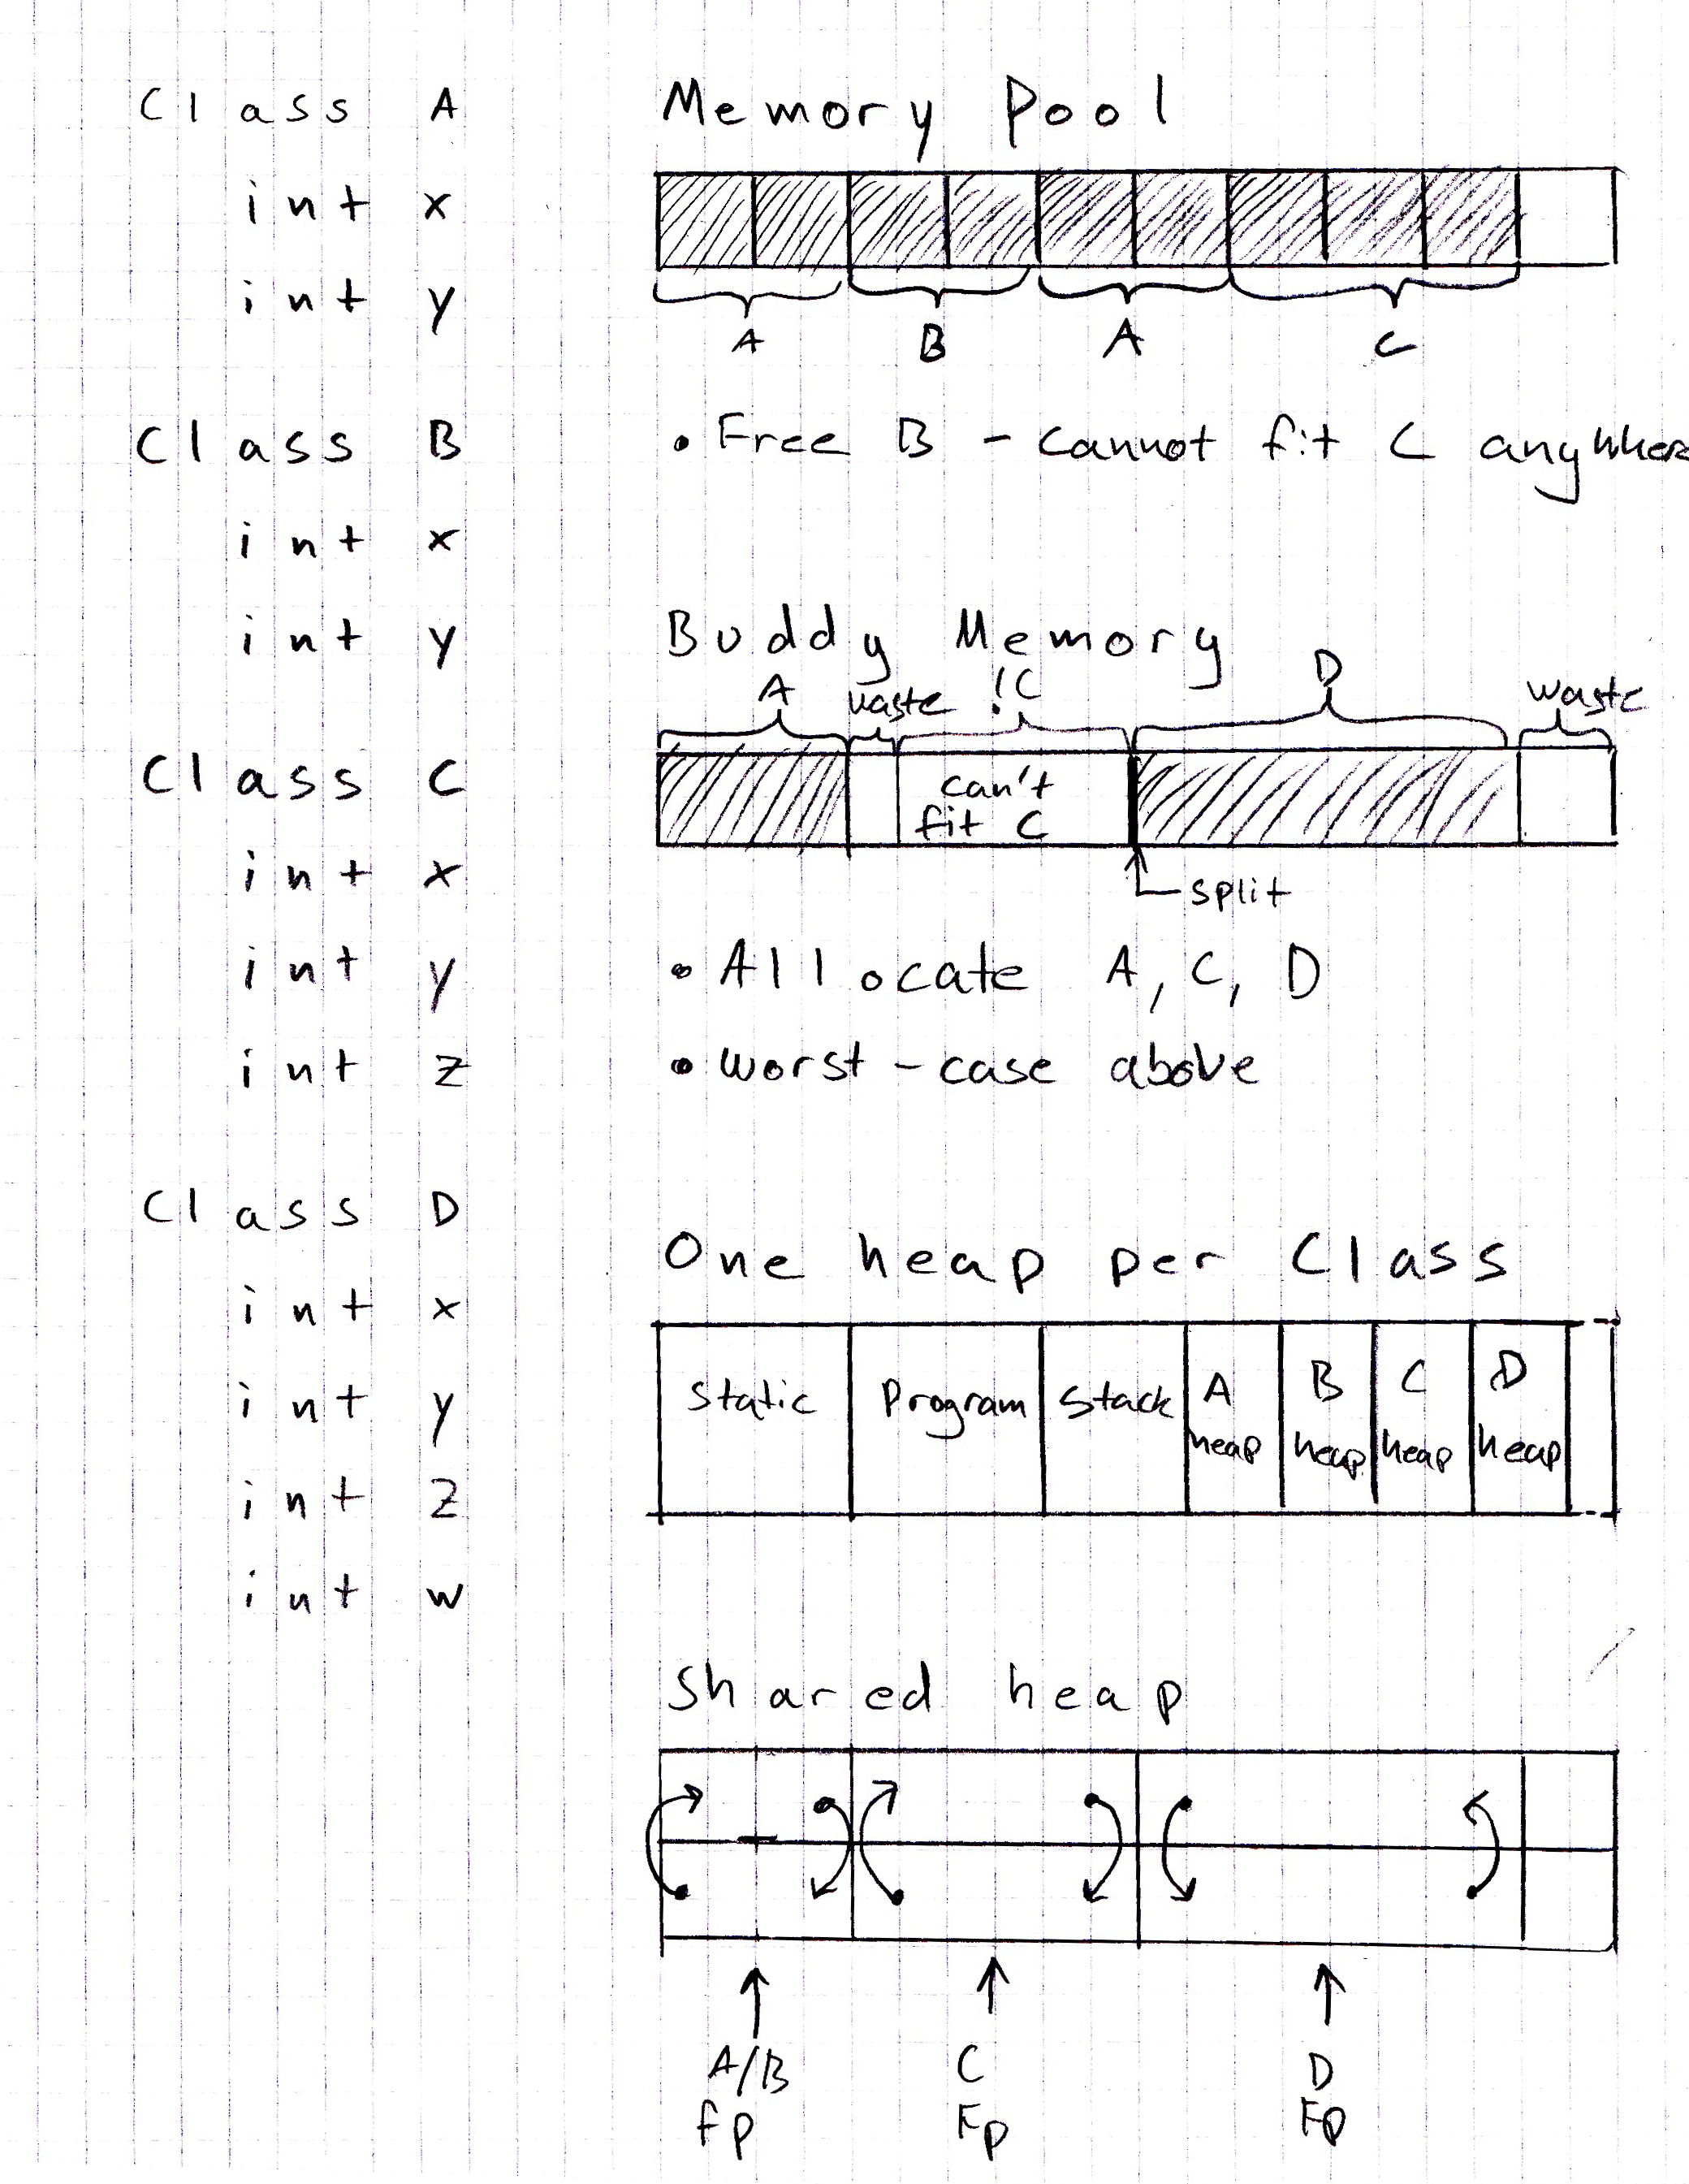
\includegraphics[width=0.7\textwidth]{heap-designs}
  \caption{Heap memory layouts (Draft)}
\end{figure}